\subsection{Tractography Reconstruction}
\label{subsec:experiments_reconstruction}
This first part will describes how to create the tractography from the raw data in DICOM format. After that, the validation of the tractography is also presented.
\subsubsection{Preprocessing}
The content of this part is from the technical report \cite{bao2012dmri}. In general, in order to perform tractography from discrete measured diffusion tensor MRI data, there are some steps as follow:

\begin{enumerate}
\item From raw data to Nifti format.
\item Reconstruction.
\item Tracking.
\item Coregistration.
\end{enumerate}

The first step is to convert from DICOM to Nifti format. End of this step, all the necessary information for tracking have been extracted from the DICOM raw data including: actual dMRI data (4D array, $(I,J,K,W)$), affine transformation, gradient vector ($‘.bvec’$) and b-value ($‘.bval’$).
From these information,we can create the \emph{tractrography}, the \emph{fractional anisotropy} (FA) volume and the \emph{mean diffusivity} (MD) volume.
A tractography is created in two steps: reconstruction and tracking. Reconstruction is about computing the information about the spatial distribution of the diffusion signal within each voxel. While tracking tries to connect many signals to form a tractography based on orientation signal of each voxel. In this paragraph, the main focus is on how to reconstruction of dMRI data.   

However, before doing reconstruction, the actual dMRI data in NIfTI image needs to extract brain image only. Because the result of scanner usually contains not only brain but also other things close to brain which can distract the processing of tracking. Brain extraction is the process of removing the skull and the rest of the head from the brain, therefore is necessary to be done before further analysis. The resulting file only contains a representation of the brain's anatomy. Brain extraction can be done with the FSL program BET (Brain Extraction Tool)~\cite{smith2002automated}. FSL\footnote{\url{http://www.fmrib.ox.ac.uk/fsl/index.html}} is a comprehensive library of analysis tools for FMRI, MRI and DTI brain imaging data.

After creating tractographies from the raw data in dicom format, the next step is coregistration. Becasue all these tractographies were initially in native space or space of scanner and every measurement has it own coordinator, it is very difficult for doctor or neuroscientist can compare, integrate or further studying them. They are needed to be warped into the common space. The goal is to warp the tractography from native space into MNI space (Montreal Neurological Institute)~\footnote{\url{http://www.mni.mcgill.ca/}}, a standard brain based on the averaging of 58 peoples. In contrast to the all the method mentioned before, in this implement we use FA registration mappings or affine transformation applied on tractography which is also most commonly used in the literature along with other tensor based methods~\cite{goh2006algebraic}. More detail can be found in \cite{bao2012dmri}

At the end of this procedure, we get the whole tractography in the common MNI cordinator. The next step is to validate the result to check the accuracy of the tractography.

\subsubsection{Validation}
This step is aimed at validation the result tractography of the previous step. We investigate on two ways. First, we try to statistic analyse the tractography of all subjects and controls to see whether there is any unusual case or not. Some features can be used such as

\begin{enumerate}
	\item Number of tracts for every subject and control
	\item Length: min, max and average
	\item Align on spagetti
\end{enumerate}

%
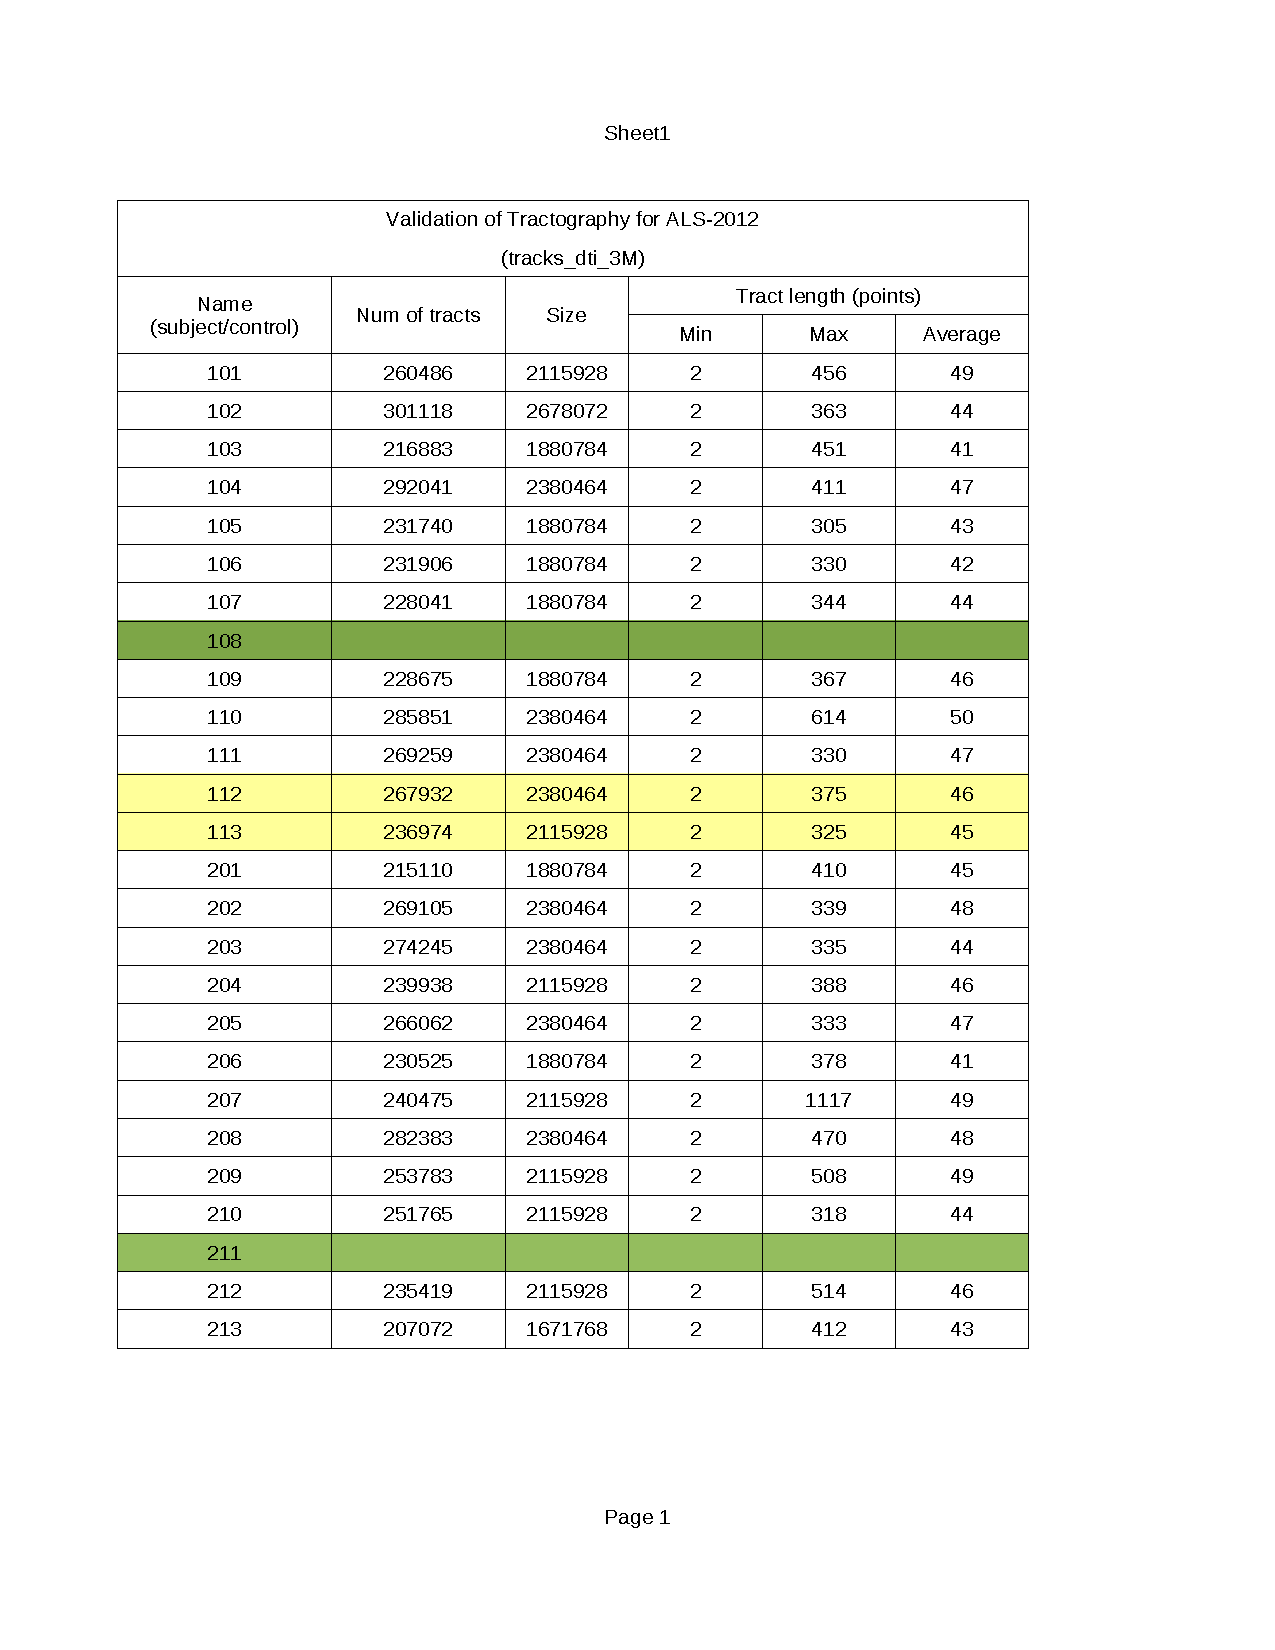
\includepdf[pages={1-3},picturecommand={Statistical features of the tractography}]{validation_120531_dti_10k.pdf}
\label{table:validation}

%\begin{figure}  
%  \centering
%  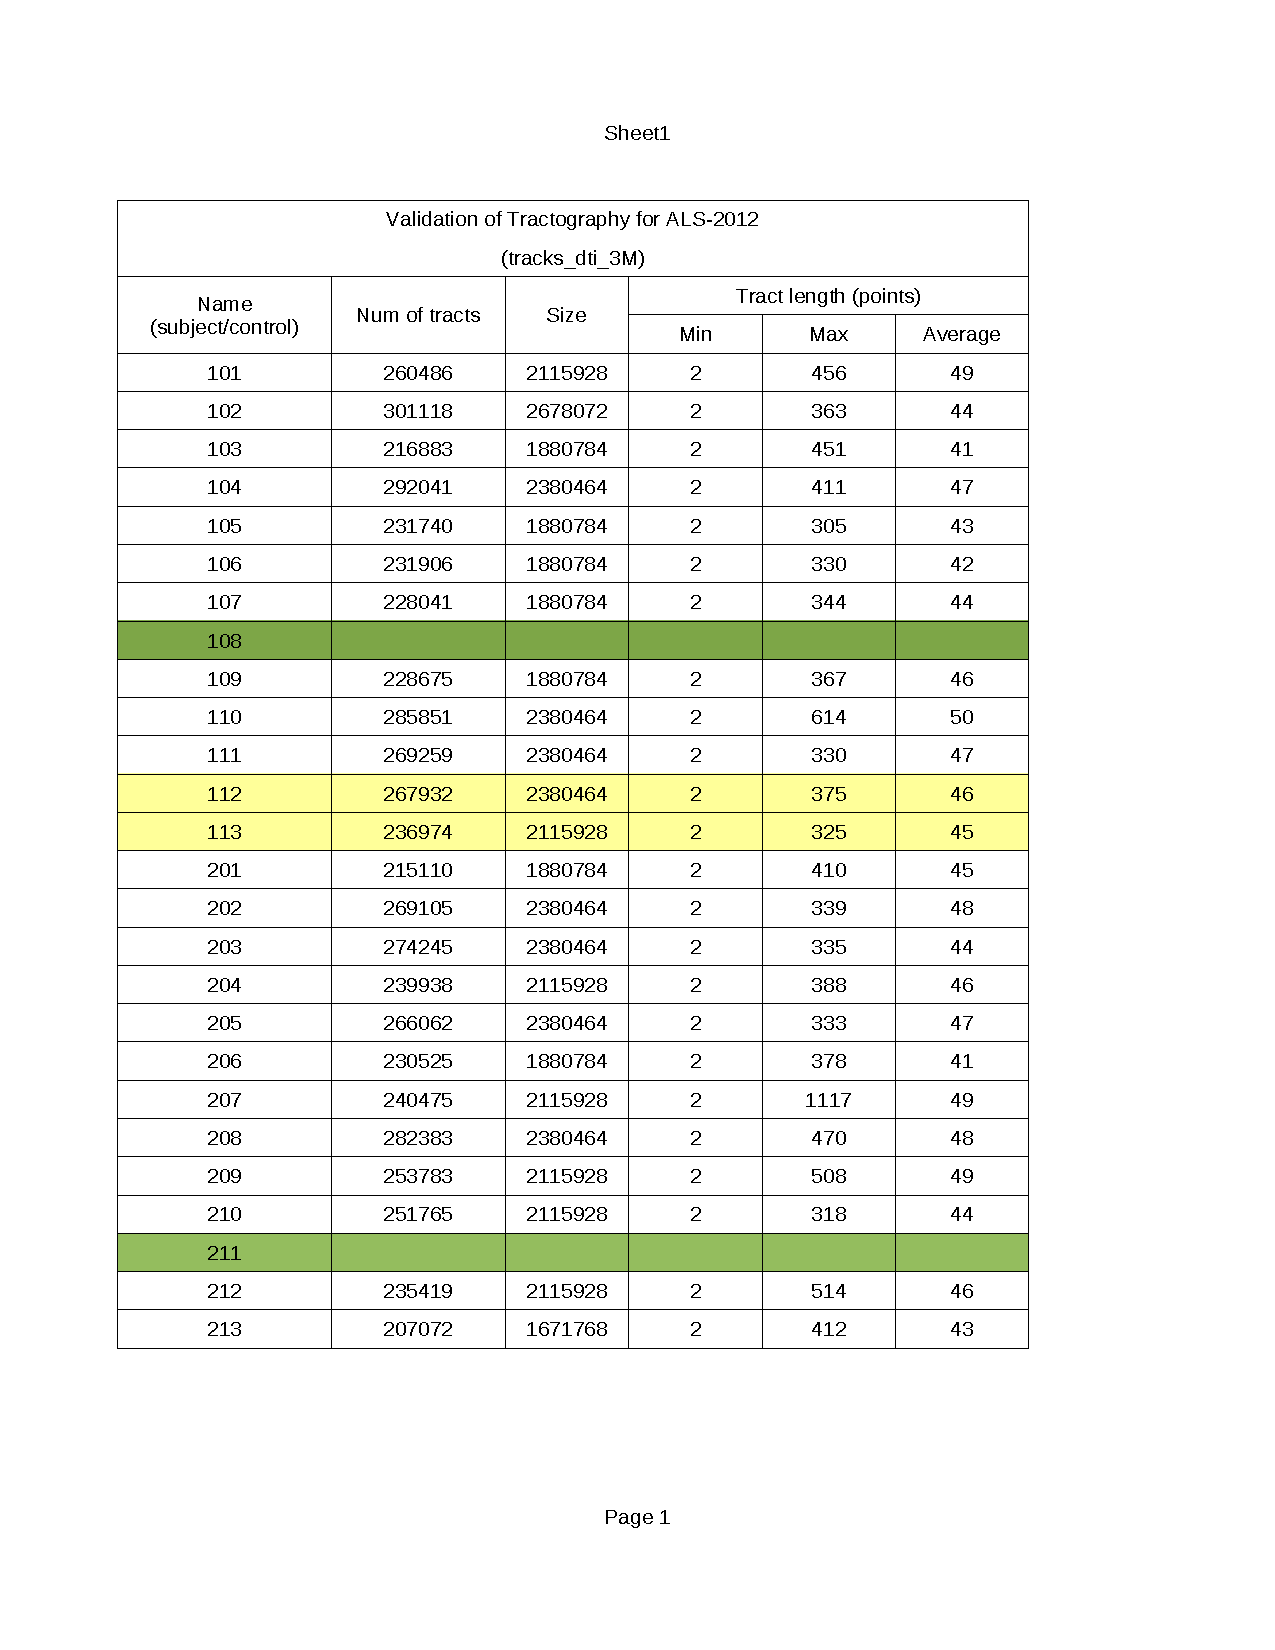
\includegraphics[width=15cm]{validation_120531_dti_10k.pdf}
%  %[bb 0 0 400 400]
%  \caption{The statistical features of tractography.}
%  \label{fig:validation}
%\end{figure}
%
The table in the \ref{table:validation} shows the statistic of some basic features of tractography. Note that, here we use $10K$, $1M$ and $3M$ seeds to create tractography and the number of tracts is about $10\%$ of the number of seeds. Later, we visualize the anatomy on FSL and align both tractography and anatomy using Sphagetti software. Both the statistically validation and visualization show that all the tractographies are coherent and in a satisfactory situation. %Otherwhile, the table of gradient is also presented in \ref{table:gradient}
